\subsubsection{Cache 分发}


\begin{figure}[H]
    \centering
    \begin{minipage}[H]{0.45\textwidth}
        \centering
        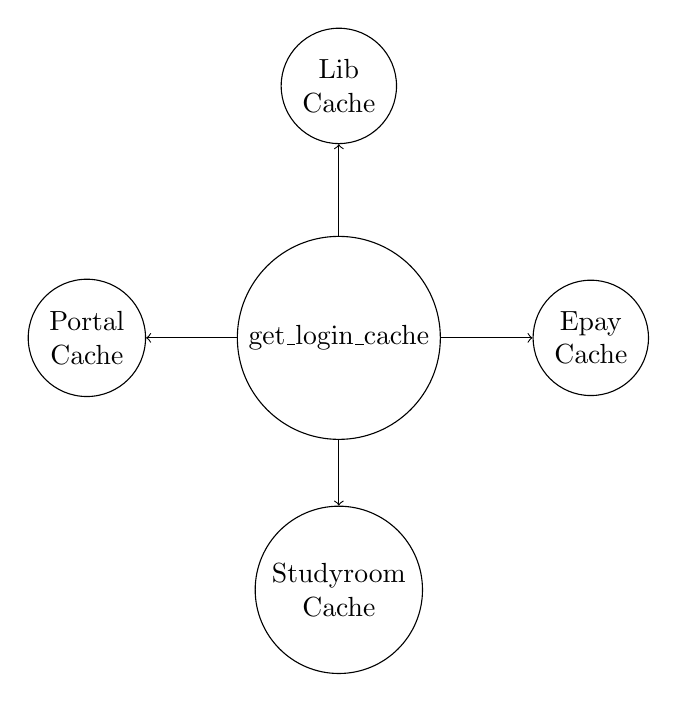
\begin{tikzpicture}[
            node distance=3.2cm,
            every node/.style={draw, circle, minimum size=1.2cm, align=center},
            every edge/.style={draw, thick, -{Latex[length=2mm, width=1mm]}}
        ]

            \node[draw] (center) {get\_login\_cache};

            \node[above of=center] (top) {Lib \\ Cache};
            \node[below of=center] (bottom) {Studyroom \\ Cache};
            \node[left of=center] (left) {Portal \\ Cache};
            \node[right of=center] (right) {Epay \\ Cache};

            \draw[->] (center) -- (top);
            \draw[->] (center) -- (bottom);
            \draw[->] (center) -- (left);
            \draw[->] (center) -- (right);

        \end{tikzpicture}
    \end{minipage}
    \hfill
    \begin{minipage}[H]{0.5\textwidth}
        \textbf{PluginLoader 缓存分发功能}:
        \begin{itemize}
            \item \textbf{Lib Cache}:用于图书馆管理系统。
            \item \textbf{Studyroom Cache}:用于研修间自动预约系统。
            \item \textbf{Portal Cache}:用于公共数据库页面的缓存,目前仅用于课表的获取。
            \item \textbf{Epay Cache}:用于华东师范大学校园卡管理页面的自动查询电费功能。
            \item \textbf{More Cache...}:适配的框架可以获取其余 ECNU 页面的 Cache 以供开发者使用。
        \end{itemize}
        \textbf{功能说明}:
        PluginLoader 是一个插件管理器,它可以加载、卸载和管理插件。
        通过调用 \texttt{get\_login\_cache()} 函数,PluginLoader 实现各缓存的分发,
        各缓存分发后供相应的插件调用。

        \vspace{0.2cm}

    \end{minipage}
\end{figure}

\begin{rmr}
    \textbf{更多适配}:
    我们已经实现了基本的 Cache 抓取框架,以供后续的开发者调用,调用示例如下:

    \texttt{get\_login\_cache(cache\_grabbers=[\{MoreCache\}.grab\_from\_driver])}
\end{rmr}

除此之外,每一个插件都拥有自己的 Routine 事件周期,Plugin 在注册时需要附带该属性,
以保证 PluginLoader 能够轮询执行插件的例行任务(通过 PluginLoader 中定义的 \texttt{poll()} 函数来执行)。

\subsubsection{基于 Routine 的事件调度逻辑}

\begin{note}
    \noindent \textbf{PluginLoader} 根据预定义的频率(Secondly、Minutely、Hourly、Daily、Weekly),调用每个插件的 \texttt{on\_routine} 方法。插件会根据任务频率接收并处理任务,完成对应的功能逻辑。

    \vspace{0.3cm}

    \noindent 箭头上的 "Routine" 统一表示调度逻辑,具体任务频率的细节由配置文件决定。例如:
    \begin{itemize}
        \item \texttt{Routine: Secondly} → 调用 插件 A 的 \texttt{on\_routine}。
        \item \texttt{Routine: Daily} → 调用 插件 D 的 \texttt{on\_routine}。
    \end{itemize}
\end{note}

\vspace{0.27cm}

\begin{center}
    \begin{tikzpicture}
        [
        plugin/.style={
            rectangle,
            draw,
            rounded corners,
            fill=orange!20,
            minimum width=1.5cm,
            minimum height=0.8cm,
            align=center
        },
        loader/.style={
            rectangle,
            draw,
            fill=blue!20,
            minimum width=3cm,
            minimum height=1cm,
            align=center
        },
        dashedbox/.style={
            draw,
            dashed,
            thick,
            rounded corners,
            inner sep=0.5cm
        },
        arrow/.style={
            ->,
            thick,
            >=Stealth
        }
        ]
        % 定义插件节点,水平排列
        \node (A) [plugin] {插件 A};
        \node (B) [plugin, right=of A] {插件 B};
        \node (C) [plugin, right=of B] {插件 C};
        \node (D) [plugin, right=of C] {插件 D};
        \node (E) [plugin, right=of D] {插件 E};

        % 使用 fit 库创建包裹插件的虚线框
        \node [dashedbox, fit=(A) (E)] (dashedbox) {};

        % 将 PluginLoader 放置在虚线框正上方并居中
        \node (loader) [loader, above=1.5cm of dashedbox] {PluginLoader.poll()};

        % Draw curved arrows from PluginLoader to each plugin
        \draw[arrow, bend right=30] (loader.south) to node[midway, sloped, above] {Routine A} (A.north);
        \draw[arrow, bend right=15] (loader.south) to node[midway, sloped, above] {Routine B} (B.north);
        \draw[arrow] (loader.south) to node [midway, sloped, above] {Routine C} (C.north); % Straight arrow for the middle plugin
        \draw[arrow, bend left=15] (loader.south) to node [midway, sloped, above] {Routine D} (D.north);
        \draw[arrow, bend left=30] (loader.south) to node [midway, sloped, above] {Routine E} (E.north);

    \end{tikzpicture}
\end{center}

\subsubsection{插件配置管理}

\begin{note}
    此部分代码如 \texttt{root/src/plugin/config.py} 所示。

    我们使用装饰器来实现插件的注册,注册信息存储于 \texttt{Registry} 类的字典中,每个插件对应着一个 \texttt{Record} 对象。
\end{note}

示例性的插件注册代码如 \texttt{root/plugins/calendar\_notice.py} 中所示:

\begin{lstlisting}[language=python]
    @register_plugin(
        name="calendar_notice",
        configuration=PluginConfig().add(
            TimeItem(
                name="notice_before_class_start", default_value=datetime.time(0, 10),
                description="上课提前提醒时间 (提前h小时m分钟)"
            )
        ),
        routine=Routine.MINUTELY,
        ecnu_cache_grabber=PortalCache.grab_from_driver
    )
\end{lstlisting}

文件中有 \texttt{PluginConfig} 和 \texttt{PluginContext} 类,它们的功能如下:

\begin{itemize}
    \item \textbf{PluginConfig}:插件的配置项集合。插件可继承 \texttt{PluginConfig} 类并添加多个 \texttt{ConfigItem} 子类来描述其配置需求。
    \item \textbf{ConfigItem}:每个配置项通过继承 \texttt{ConfigItem} 类及其子类(如 \texttt{TextItem}、\texttt{NumberItem} 等)来定义。
\end{itemize}

\textbf{功能说明}:PluginConfig 提供了一种结构化的方式来定义插件的配置项,支持配置项的序列化和反序列化,方便配置的保存和加载。
插件在注册时通过 \texttt{PluginConfig} 指定其需要的配置项,框架会自动处理配置的管理。

\begin{figure}[H]
    \centering
    \resizebox{0.4\textwidth}{!}{
        \begin{tikzpicture}
            [
            pluginconfig/.style={ rectangle, draw, rounded corners, fill=green!20, minimum width=3cm, minimum height=1cm, align=center },
            configitem/.style={ rectangle, draw, rounded corners, fill=yellow!20, minimum width=2cm, minimum height=0.8cm, align=center },
            dashedbox/.style={ draw, dashed, thick, rounded corners, inner sep=0.5cm },
            arrow/.style={ ->, thick, >=Stealth }
            ]
            \node (pluginconfig) [pluginconfig] {PluginConfig};
            \node (textitem) [configitem, below left=of pluginconfig] {TextItem};
            \node (numberitem) [configitem, below=of pluginconfig] {NumberItem};
            \node (dateitem) [configitem, below right=of pluginconfig] {DateItem};

            \node [dashedbox, fit=(textitem) (numberitem) (dateitem)] (dashedbox) {};

            \draw[arrow] (pluginconfig) -- (textitem);
            \draw[arrow] (pluginconfig) -- (numberitem);
            \draw[arrow] (pluginconfig) -- (dateitem);

        \end{tikzpicture}
    }
    \caption{PluginConfig 和 ConfigItem 的关系示意图}
\end{figure}

\subsubsection{插件上下文管理}

此部分代码见 \texttt{root/src/plugin/context.py} 所示。

\begin{note}
    为了保证项目的整洁和规范性,插件创建文件和记录日志等操作请使用生命周期函数和事件函数中提供的 PluginContext 进行。
    它为每个插件提供了一个上下文环境,使插件能够与框架进行交互和访问必要的资源。
\end{note}

\begin{figure}[H]
    \centering
    \resizebox{0.95\textwidth}{!}{
        \begin{minipage}[H]{0.4\textwidth}
            \centering
            \begin{tikzpicture}
                [
                context/.style={
                    rectangle,
                    draw,
                    rounded corners,
                    fill=red!20,
                    minimum width=3cm,
                    minimum height=1cm,
                    align=center
                },
                feature/.style={
                    rectangle,
                    draw,
                    rounded corners,
                    fill=white!80,
                    minimum width=2.5cm,
                    minimum height=0.8cm,
                    align=center
                },
                arrow/.style={
                    ->,
                    thick,
                    >=Stealth
                }
                ]

                % PluginContext Node
                \node (context) [context] {PluginContext};

                % Features of PluginContext
                \node (logger) [feature, above left=of context] {日志记录器};
                \node (cache) [feature, above right=of context] {插件缓存};
                \node (message) [feature, below left=of context] {消息传递};
                \node (actions) [feature, below right=of context] {用户操作绑定};

                % Arrows from PluginContext to Features
                \draw[arrow] (context) -- (logger);
                \draw[arrow] (context) -- (cache);
                \draw[arrow] (context) -- (message);
                \draw[arrow] (context) -- (actions);

            \end{tikzpicture}
        \end{minipage}
        \hspace{2.5cm}
        \begin{minipage}[H]{0.6\textwidth}
            \textbf{PluginContext 的功能组成}:
            \begin{itemize}
                \item \textbf{日志记录}:
                插件专属的日志记录(信息、警告、错误等)。
                \item \textbf{插件缓存}:
                插件可以通过 \texttt{ctx.get\_cache()} 访问自己的持久化缓存,用于存储跨会话的数据。
                缓存支持数据的读取和写入,确保插件状态的持久性。
                \item \textbf{消息传递}:
                允许插件间通信。
                \item \textbf{用户操作绑定}:
                插件可以绑定用户界面的操作(如按钮),相应的回调函数相应用户的操作。
            \end{itemize}
        \end{minipage}
    }
\end{figure}
